\section{Pianificazione}

Al fine della pianificazione si è deciso di suddividere il progetto in cinque macro-fasi distinte:
\begin{itemize}
\item \textbf{Analisi:} incentrata maggiormente sull'analisi dei requisiti;
\item \textbf{Incremento fase di Analisi:} incentrata sul consolidamento dei requisiti;
\item \textbf{Progettazione Architetturale:}
\item \textbf{Progettazione di dettaglio e codifica:}
\item \textbf{Verifica e Validazione:}
\end{itemize}
Ogni macro-fase è stata poi suddivisa in varie attività a loro volta scomposte in sotto-attività ancora più di dettaglio ad ognuna delle quali sono assegnate una o più risorse. La dislocazione temporale delle attività è evidenziata attraverso diagrammi di \glossario{Gantt} per rappresentarne la durata, la sequenzialità e il parallelismo. Tali diagrammi includono anche:
\begin{itemize}
\item \textbf{\glossario{Milestone}:} rappresenta la data prevista per la conclusione dell'attività e coincide con la data della consegna dei documenti in vista della revisione associata;
\item \textbf{Attività che compongono la macro-fase:} suddivise poi in sotto attività.
\end{itemize}
Si è scelto di non riportare i diagrammi \glossario{PERT} in quanto, a causa della eccessiva quantità di nodi, si sono rivelati poco leggibili. I grafici \glossario{WBS} evidenziano la struttura gerarchica delle attività: di che attività si compone ogni macro-fase e le sotto-attività di cui ogni attività è composta, tutte univocamente identificate 

\subsection{Analisi}
\textbf{Periodo:} da 2015-12-18 a 2016-01-22 \\
Tale fase inizia in corrispondenza della data di scadenza per la formazione dei gruppi e termina con la data di consegna dei documenti per la revisione dei requisiti. La fase di \textbf{Analisi} prevede la seguente scomposizione in attività:
\begin{itemize}
\item \textbf{Norme di Progetto:} l'\textit{Amministratore} si occupa di redigere ed emanare le norme che tutti i componenti del gruppo dovranno rispettare nello svolgersi dell'intero progetto. Le \textit{Norme di Progetto} sono il primo documento ad essere prodotto in quanto regolano anche la stesura dei documenti e l'utilizzo del software di supporto necessarie già in questa prima fase. Sarà compito dei \textit{Verificatori} assicurare il rispetto di tali norme.
\item \textbf{Studio di Fattibilità:} a seguito della valutazione di tutti i capitolati viene redatto \textit{Studio di Fattibilità}. Si tratta di un documento ad uso interno in cui viene studiata la complessità delle varie proposte. La redazione e approvazione di tale documento condiziona l'inizio dell'\textit{Analisi dei Requisiti}.
\item \textbf{Piano di Progetto:} il \textit{Responsabile} del gruppo è tenuto a redigere in questa fase il \textit{Piano di Progetto} contenente la pianificazione così da organizzare le attività del gruppo.
\item \textbf{Analisi dei Requisiti:} viene generata un'analisi più approfondita, rispetto allo \textit{Studio di Fattibilità}, nell'\textit{Analisi dei Requisiti}. Questa attività continua fino alla data di consegna della documentazione.
\item \textbf{Piano di Qualifica:} \textit{Progettista} e \textit{Verificatore} redigono il \textit{Piano di Qualifica}.
\item \textbf{Lettera di Presentazione:} si tratta di una lettera redatta su carta intestata da presentare al Committente che permette al gruppo di partecipare alla gara d'appalto per il capitolato scelto.
\item \textbf{Glossario:} viene scritto in modo incrementale dai redattori dei documenti. Esso contiene la spiegazione di alcuni termini, opportunamente contrassegnati con un G pedice, contenuti all'interno della documentazione. Viene aggiornato passo passo ad ogni aggiunta di termini che necessitano di spiegazione.
\end{itemize}
Nella fase di Analisi i ruoli maggiormente coinvolti sono \textit{Analista}, \textit{Responsabile}, \textit{Amministratore} e \textit{Verificatore}.

\subsubsection{Gantt attività}
\begin{figure}[H]
\centering
\scalebox{0.3}{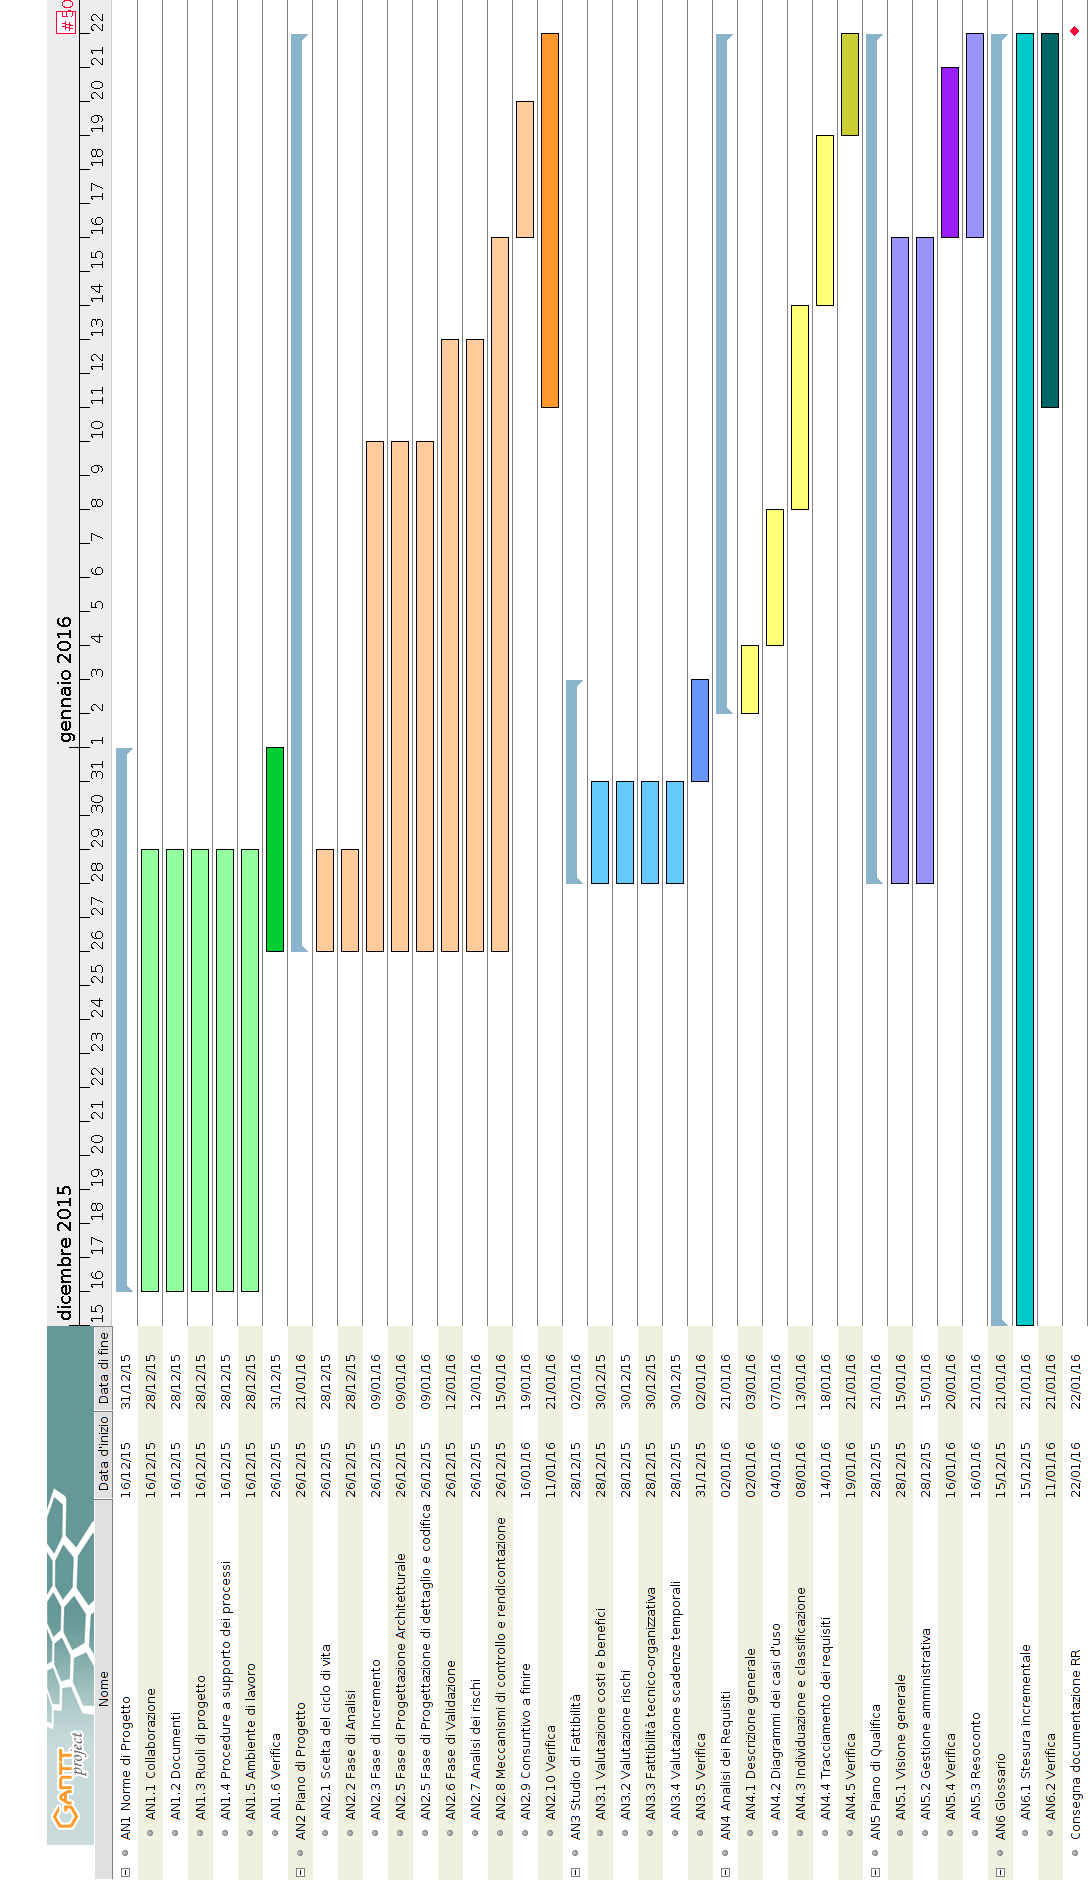
\includegraphics{gantt/ganttAnalisi.png}}
\caption{Diagramma di Gantt, fase di Analisi}
\end{figure}

\subsubsection{WBS attività}
\begin{figure}[H]
	\centering
    \scalebox{0.8}{\pgfdeclarelayer{bg}    % declare background layer
\pgfsetlayers{bg,main}  % set the order of the layers (main is the standard layer)

\tikzset{
every node/.style={draw,text width=2cm},
style1/.style= {rectangle, thin, align=center, fill=gray!20, text width=5cm},
style2/.style= {rectangle, thin, align=left,yshift=-2cm, text width=4cm}
}



\begin{tikzpicture}[
remember picture,
level 1/.style={sibling distance=50mm},
edge from parent/.style={->,draw,thick},
>=latex]

% the initial tree ("root" and "text nodes")
\node[style1] (1) {AN1 Norme di Progetto}
child {node[style2] (c1) {AN1.1 Collaborazione}}
child {node[style2] (c2) {AN1.2 Documenti}}
child {node[style2] (c3) {AN1.3 Ruoli di progetto}}
child {node[style2, below of=c1] (c4) {AN1.4 Procedure a supporto dei processi}}
child {node[style2, below of=c2] (c5) {AN1.5 Ambiente di lavoro }}
child {node[style2, below of=c3] (c6) {AN1.6 Verifica}};

 \begin{pgfonlayer}{bg}
    \path[every node/.style={font=\sffamily\small}]
    (1) edge (c4)
        edge (c5)
        edge (c6);
  \end{pgfonlayer}


\end{tikzpicture}



}
\end{figure}

\subsubsection{Ripartizione ore}
Per il glossario non è stata prevista alcuna ripartizione delle ore tra i componenti del gruppo per la redazione in quanto viene redatto contemporaneamente alla stesura degli altri documenti ogni qualvolta un termine necessiti di una spiegazione.
\bgroup
\begin{longtable}{|l|l|l|c|}
  \endfirsthead
  \hline
  \textbf{Identificativo} &
  \textbf{Nome Attività} &
  \textbf{Ruolo} &
  \textbf{Ore}\\
  \endhead
  \hline
  \textbf{AN1} & \textbf{Norme di Progetto} &  &  \\
  \hline
  	{AN1.1} & Collaborazione & Amministratore  & 4\\
  	\hline
  	{AN1.2} & Documenti & Amministratore & 4\\
  	\hline
  	{AN1.3} & {Ruoli di progetto} & Amministratore &  0.5\\
  	\hline
  	{AN1.4} & {Procedure a supporto dei processi} & Amministratore  &  3\\
  	\hline
  	{AN1.5} & {Ambiente di lavoro} & Amministratore &  4\\
  	\hline
  	{AN1.6} & {Verifica} & Verificatore & 3 \\
  \hline
  \textbf{AN2} & \textbf{Piano di Progetto}  & & \\
    \hline
    	{AN2.1} & {Scelta del ciclo di vita} & Responsabile &  2\\
    	\hline
    	{AN2.2} & {Fase di Analisi} & Responsabile& 3 \\
    	\hline
    	{AN2.3} & {Fase di Incremento} & Responsabile& 2 \\
    	\hline
    	{AN2.4} & {Fase di Progettazione Architetturale} & Responsabile &   3\\
    	\hline
    	{AN2.5} & {Fase di Progettazione di dettaglio e codifica} & Responsabile  &  3\\
    	\hline
    	{AN2.6} & {Fase di Verifica e Validazione} & Responsabile  &  3\\
    	\hline
    	{AN2.7} & {Analisi dei rischi} & Responsabile  &  3\\
    	\hline
    	{AN2.8} & {Meccanismi di controllo e rendicontazione} & Responsabile & 2\\
    	\hline
    	{AN2.9} & {Consuntivo a finire} & Verificatore1  & 3\\
    	\hline
    	{AN2.10} & {Verifica} & Verificatore2  & 3 \\
    \hline
    \textbf{AN3} & \textbf{Studio di Fattibilità}  & &  \\
      \hline
      	{AN3.1} & {Valutazione costi e benefici} & Analista1  & 3 \\
      	\hline
      	{AN3.2} & {Valutazione rischi} & Analista2 & 3\\
      	\hline
      	{AN3.3} & {Fattibilità tecnico-organizzativa} & Analista3  & 3 \\
      	\hline
      	{AN3.4} & {Valutazione scadenze temporali} & Analista4  & 3 \\
      	\hline
      	{AN3.5} & {Verifica} & Verificatore  & 2 \\
      \hline
      \textbf{AN4} & \textbf{Analisi dei Requisiti} & &  \\
         \hline
         {AN4.1} & {Descrizione generale} & Analista1  &  3\\
         & & Analista2 & 3\\
         & & Analista3 & 3\\
         \hline
         {AN4.2} & {Diagrammi dei casi d'uso} & Analista1  &  3\\
         & & Analista2 & 3\\
         & & Analista3 & 3\\
         \hline
         {AN4.3} & {Individuazione e classificazione} & Analista1  &  5\\
         & & Analista2 & 5\\
         & & Analista3 & 5\\
         \hline
         {AN4.4} & {Tracciamento dei requisiti} & Analista1  &  2\\
         & & Analista2 & 2\\
         & & Analista3 & 2\\
         \hline
         {AN4.5} & {Verifica} & Verificatore1  &  3\\
         & & Verificatore2 & 3\\
     \hline
     \textbf{AN5} & \textbf{Piano di Qualifica} & &  \\
         \hline
         {AN5.1} & {Visione generale} & Analista1 &  6 \\
         & & Verificatore1 & 6\\
         \hline
         {AN5.2} & {Gestione amministrativa} & Amministratore1  &  3\\
         & & Amministratore2 & 3\\
         & & Analista2 & 6\\
         & & Verificatore2 & 6\\
         \hline
         {AN5.3} & {Resoconto} & Verificatore1 &  3\\
         \hline
         {AN5.4} & {Verifica} & Verificatore2 &  3 \\
     \hline
     \textbf{AN6} & \textbf{Glossario} & &  \\
         \hline
         {AN6.1} & {Verifica} & Verificatore &  3 \\
         \hline
     \caption{Ripartizione ore fase di Analisi}
\end{longtable}
\egroup
  
\subsection{Incremento fase di Analisi}
\subsubsection{Gantt attività}

\subsubsection{WBS attività}

\subsubsection{Ripartizione ore}

\subsection{Progettazione Architetturale}
\subsubsection{Gantt attività}

\subsubsection{WBS attività}

\subsubsection{Ripartizione ore}

\subsection{Progettazione di dettaglio e codifica}
\subsubsection{Gantt attività}

\subsubsection{WBS attività}

\subsubsection{Ripartizione ore}

\subsection{Verifica e Validazione}
\subsubsection{Gantt attività}

\subsubsection{WBS attività}

\subsubsection{Ripartizione ore}